\chapter{Apéndice B: Documentación-ROTAX}
    La información presentada aquí es el certificado de Aeronavegabilidad y documentación técnica del motor trabajado en este proyecto (Motor ROTAX 912 ULS). Para presentar la bases de información que utilizamos para este proyecto respecto a los parámetros. A continuación se va adjuntar las fuentes de adquisición de dichos documentos y fragmentos de estos mismos:
    
\begin{itemize}
    \item Certificado de Aeronavegabilidad: 
    \href{https://www.seguridadaerea.gob.es/sites/default/files/HD%20TC286-I%20r8.pdf}{www.seguridadaerea.gob.es} \\
        \hyperlink{certificado-aeronavegabilidad}{-Salto a pagina-} % Enlace directo a la primera página del certificado
    
    \item Documentación Técnica 
        \href{https://www.flyrotax.com/p/service/technical-documentation}{www.flyrotax.com} \\

    \begin{itemize}
        \item SERVICE INSTRUCTION - PAC (Pag. 8) 
            \hyperlink{service-instruction-pag8}{-Salto a pagina-} % Enlace directo a la página 8 en el documento
    \end{itemize}

    \begin{itemize}
        \item MAINTENANCE MANUAL LINE (Pag. x)
    \end{itemize}

    \begin{itemize}
        \item OPERATORS MANUAL LINE (Pag. x)
    \end{itemize}

    \begin{itemize}
        \item MAINTENANCE MANUAL (Pag. x)
    \end{itemize}

    \begin{itemize}
        \item USER MANUAL (Pag. x)
    \end{itemize}
\end{itemize}

% Insertar el PDF completo a continuación de la descripción
\begin{landscape}
    % Insertar el PDF del certificado y establecer un marcador en la primera página
    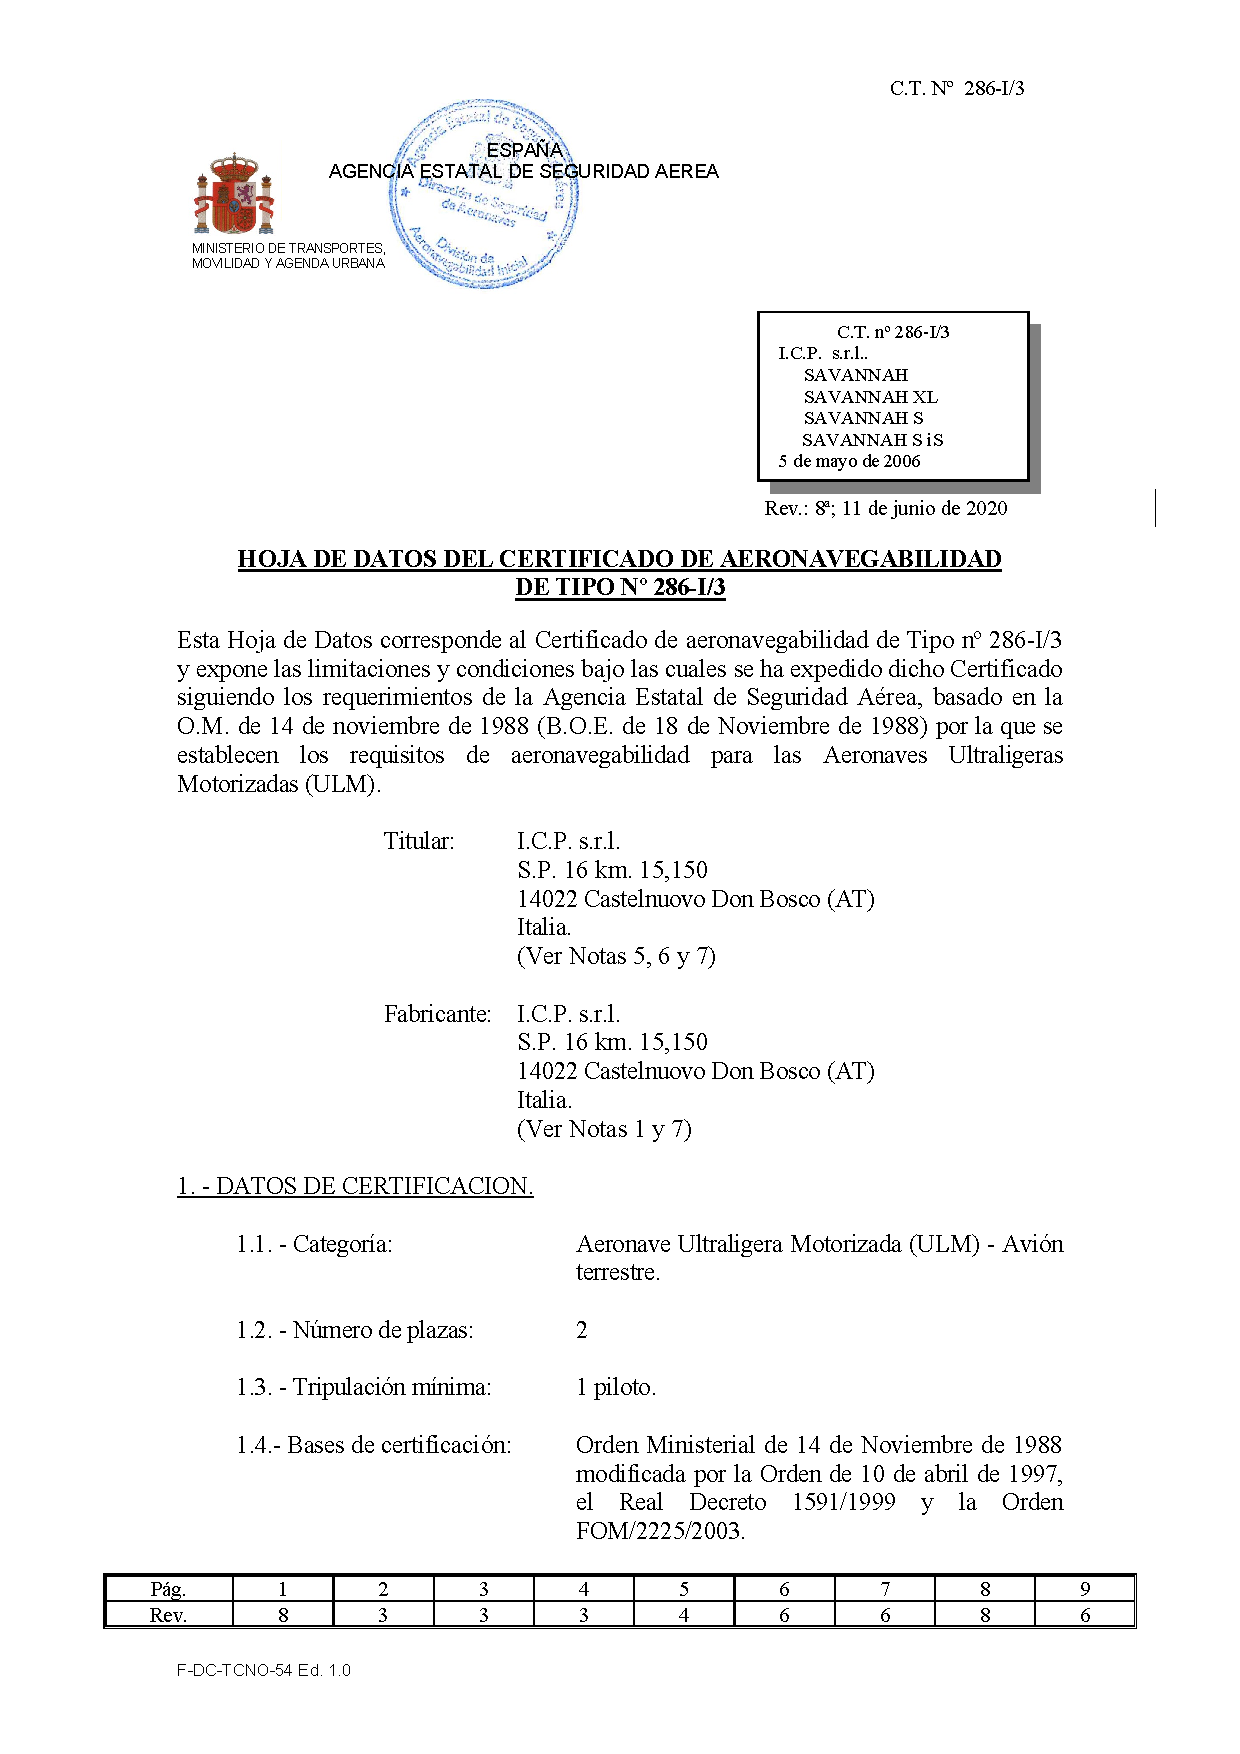
\includepdf[pages=1-9, scale=0.9, pagecommand={\hypertarget{certificado-aeronavegabilidad}{}}]{Anexo-B Bloque/HD TC286-I r8.pdf}
    % Este es el Certificado de Aeronavegabilidad con el marcador para el enlace
\end{landscape}

\begin{landscape}
    % Insertar el PDF del Service Instruction con marcador en la página 6
    \includepdf[pages=6, scale=0.9, pagecommand={\hypertarget{service-instruction-pag8}{}}]{Anexo-B Bloque/SI-PAC-027.pdf}
    % Este es el Service Instruction en la página 6 con el marcador para el enlace
\end{landscape}